\begin{figure}[!b]
\vspace{-4mm}
\begin{subfigure}{0.495\linewidth}
\centering
\includegraphics[width=\linewidth]{Images/advection_time2.pdf}
\vspace{-3mm}
\caption{Costs of particle advection.}
\label{fig:advection}
\end{subfigure}
\begin{subfigure}{0.495\linewidth}
\centering
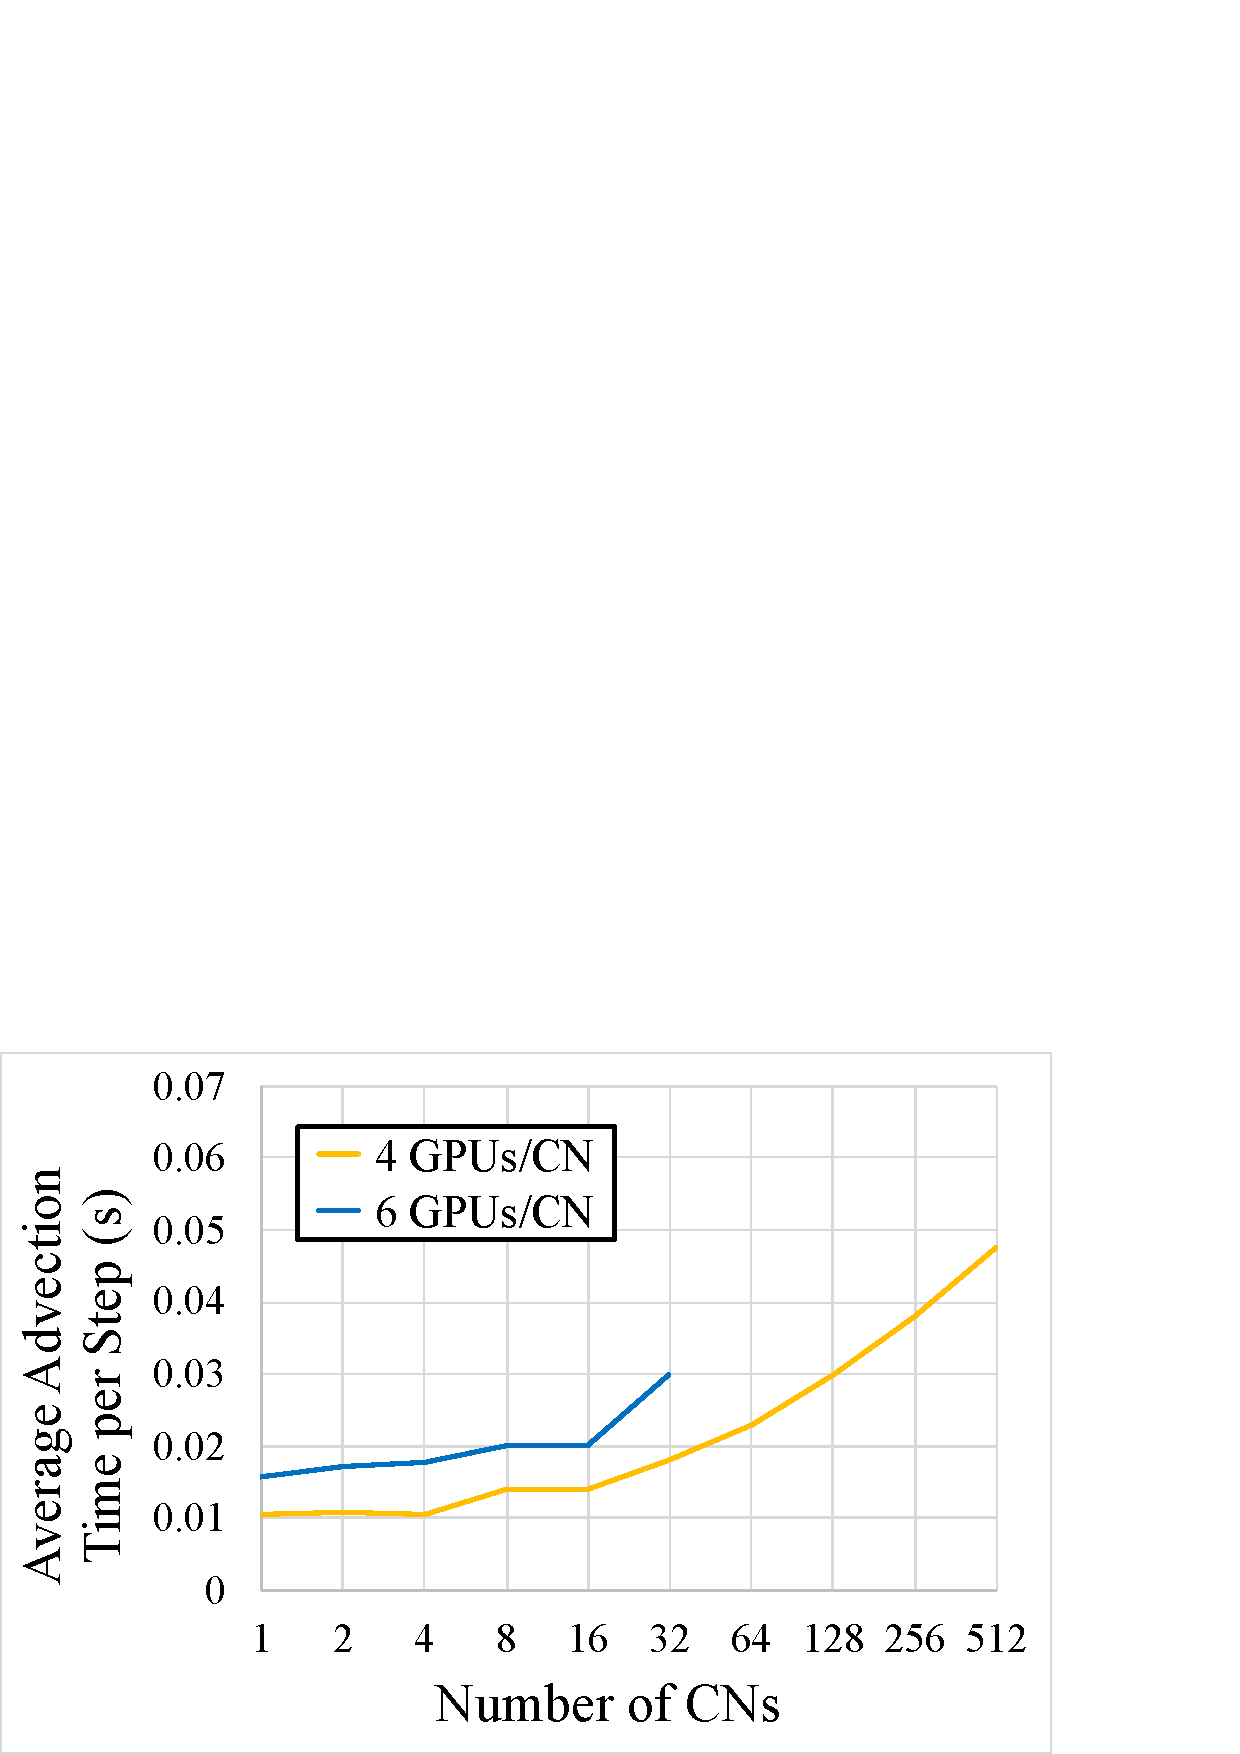
\includegraphics[width=\linewidth]{Images/communication_time2.pdf}
\vspace{-3mm}
\caption{Costs of communication.}
\label{fig:communication}
\end{subfigure}
\caption{\fix{Results for weak scaling the number of GPUs or ranks (4 or 6) per compute node. Lagrangian$_{Local}$ particle advection and Lagrangian$_{Dist}$ communication costs are used in~\ref{fig:advection} and~\ref{fig:communication}, respectively. Although particle advection performed better with fewer GPUs sharing memory on a single compute node, communication benefitted from MPI optimizations when more ranks execute on a single compute node.}} 
\label{fig:gpu_nodes}
\end{figure}
